\documentclass[UTF8]{ctexart}
\usepackage[colorlinks=true]{hyperref}

\usepackage{amsmath, bm,amsfonts}
\usepackage{hyperref}
\usepackage[normalem]{ulem}
% \usepackage{enumitem}
% \setlist{nosep}
\usepackage{caption}
\usepackage{graphicx}
% \graphicspath{{./pic/}}
\usepackage[usenames, dvipsnames]{xcolor}
\usepackage{listings}
% settings for listings.sty
\renewcommand{\lstlistingname}{代码清单}
\lstdefinestyle{lfonts}{
  basicstyle   = \footnotesize\ttfamily,
  stringstyle  = \color{purple},
  keywordstyle = \color{blue!60!black}\bfseries,
  commentstyle = \color{olive}\scshape,
}
\lstdefinestyle{lnumbers}{
  numbers     = left,
  numberstyle = \tiny,
  numbersep   = 1em,
  firstnumber = 1,
  stepnumber  = 1,
}
\lstdefinestyle{llayout}{
  breaklines       = true,
  tabsize          = 2,
  columns          = flexible,
}
\lstdefinestyle{lgeometry}{
  xleftmargin      = 15pt,
  xrightmargin     = 0pt,
  frame            = tb,
  framesep         = \fboxsep,
  framexleftmargin = 15pt,
}
\lstdefinestyle{lgeneral}{
  style = lfonts,
  style = lnumbers,
  style = llayout,
  style = lgeometry,
}
\def\beginlstdelim#1#2#3{%
  \def\endlstdelim{#2\egroup}%
  \ttfamily#1\bgroup\color{#3}\aftergroup\endlstdelim}
\lstdefinestyle{ldelims}{
  moredelim = **[is][\beginlstdelim{\$}{\$}{orange}]{\$}{\$},
  moredelim = **[is][\beginlstdelim{\{}{\}}{ForestGreen}]{\{}{\}},
  moredelim = **[is][\beginlstdelim{[}{]}{cyan}]{[}{]},
}
% LaTeX lst style
\lstdefinestyle{lltx}{
  language = {[LaTeX]TeX},
  style = lgeneral,
  style = ldelims,
  morekeywords = {% LaTeX original commands
    maketitle,
    rmfamily, sffamily, ttfamily,
    itshape, slshape, scshape,
    mdseries, bfseries, emph,
    textrm, textsf, texttt,
    textit, textsl, textsc,
    textmd, textbf,
    newcommand, renewcommand, providecommand,
    cs, meta, marg, oarg, parg
  }
}
\lstdefinestyle{iltx}{
  style      = lltx,
  basicstyle = \ttfamily
}
\lstdefinestyle{lbash}{
  language   = {bash},
  style      = lgeneral,
}
\lstdefinestyle{ibash}{
  style      = lbash,
  basicstyle = \ttfamily
}

% code style setting
\definecolor{codegreen}{rgb}{0,0.6,0}
\definecolor{codegray}{rgb}{0.5,0.5,0.5}
\definecolor{codepurple}{rgb}{0.58,0,0.82}
\definecolor{backcolour}{rgb}{0.95,0.95,0.92}

\lstdefinestyle{mystyle}{
	backgroundcolor=\color{backcolour},   
	commentstyle=\color{codegreen},
	keywordstyle=\color{magenta},
	numberstyle=\tiny\color{codegray},
	stringstyle=\color{codepurple},
	basicstyle=\footnotesize,
	breakatwhitespace=false,         
	breaklines=true,                 
	captionpos=b,                    
	keepspaces=true,                 
	numbers=left,                    
	numbersep=5pt,                  
	showspaces=false,                
	showstringspaces=false,
	showtabs=false,                  
	tabsize=2
}
\endinput

\usepackage{hologo}
\usepackage{subfigure}
\usepackage{changepage}

\ctexset{
    section = {
        titleformat = \raggedright,
        name = {第,节},
        number = \chinese{section}
    }
}

\title{mmdetection解析}
\author{Sisyphes,yehao}
\date{2019年8月1日}

\begin{document}
\maketitle
\tableofcontents
\newpage

% \include{lang-natural}
% \include{lang-computer}
% \section{已有资源}
% \href{https://heary.cn/}{基于PyTorch的开源目标检测系统},
% \href{https://nicehuster.github.io/2019/04/08/mmdetection/}{mmdetection解析},
% \href{https://blog.csdn.net/weicao1990/article/details/95332938}{mmdetection源码阅读笔记},
% \href{http://spytensor.com/index.php/archives/53/}{奇淫技巧}.
\section{结构设计}
\begin{itemize}
	\item BackBone:特征提取骨架网络,ResNet,ResneXt等.
	\item Neck: 连接骨架和头部.多层级特征融合,FPN,BFP等.
	\item DenseHead:处理特征图上的密集框部分, 主要分AnchorHead, AnchorFreeHead两大类,分别有RPNHead, SSDHead,RetinaHead和FCOSHead等.
	\item RoIExtractor:汇集不同层级的特征框,将其大小统一,为二步定位,类别优化服务.
	\item RoIHead (BBoxHead/MaskHead):类别分类或位置回归等.
	\item OneStage: BackBone + Neck + DenseHead
	\item TwoStage: BackBone + Neck  + (DenseHead) + RoIExtractor + RoIHead
	
\end{itemize}


\noindent 代码结构:\\
configs 网络组件结构等配置信息\\
tools:训练和测试的最终包装\\
mmdet:
\begin{adjustwidth}{0.5cm}{0cm}
	apis: 分布式环境设定,推断和训练基类代码\\
	core: anchor,bbox,mask等在训练前和训练中的各种变换函数\\
	datasets:coco和voc格式的数据类以及一些增强代码\\
	models:模型组件,采用注册和组合构建的形式完成模型搭建\\
	ops:优化加速代码,包括nms,roialign,dcn,gcb,mask,focal\_loss等\\
\end{adjustwidth}

\begin{figure}[htbp]
	\centering
	\begin{minipage}[t]{0.48\textwidth}
	\centering
	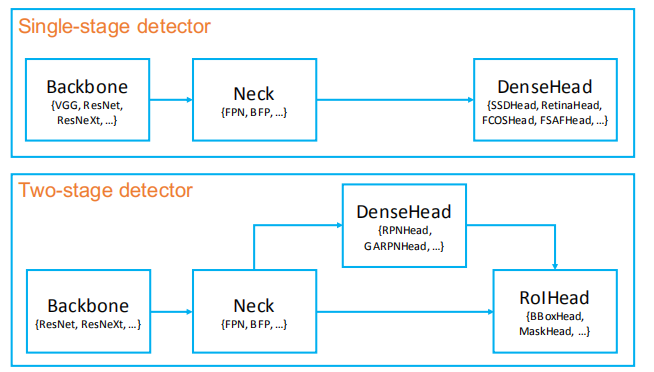
\includegraphics[width=5cm, height=3cm]{./pic/mmdetect.png}
	\caption{ Framework }
	\end{minipage}
	\begin{minipage}[t]{0.48\textwidth}
	\centering
	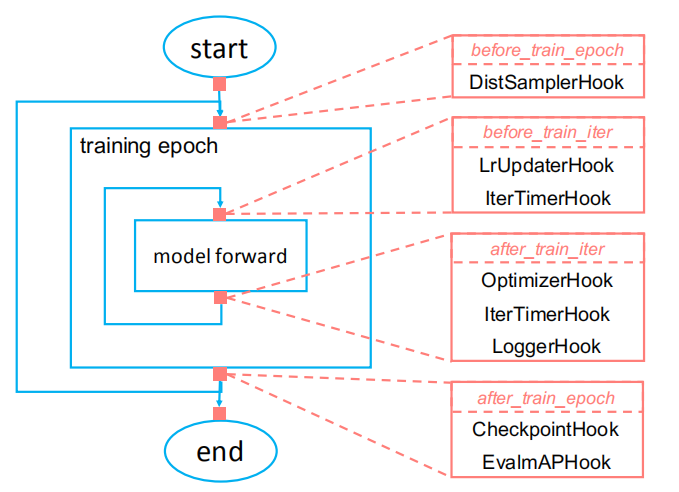
\includegraphics[width=5cm,height=3cm]{./pic/mmdetect_pipe.png}
	\caption{Trainning pipeline}
	\label{trainpipe_pic}
	\end{minipage}
\end{figure}

% \newpage
\subsection{总体逻辑}
在最外层的train.py中能看到:\\
1. mmcv.Config.fromfile从配置文件解析配置信息,并做适当更新,包括预加载模型文件,分布式相关等\\
2. mmdet.models.builder 中的build\_detector根据配置信息构造模型

\begin{adjustwidth}{0.5cm}{0cm}

2.5 build函数调用\_build\_module(新版为build\_from\_cfg)函数,按type关键字从注册表中获取相应的
模型对象,并根据配置参数实例化对象(配置文件的模型参数只占了各模型构造参数的一小部分,模型结构并非可以随意更改).\\
2.6 registr.py实现了模型的注册装饰器,其主要功能就是将各模型组件类对象保存到registry.module\_dict中,从而可以实现2.5所示功能.\\
2.7 目前包含BACKBONES,NECKS,ROI\_EXTRACTORS,SHARED\_\\
HEADS,HEADS,LOSSES,DETECTORS七个(容器).注册器可按@N
AME.register\_module方式装饰,新增.所有被注册的对象都是一个完整的pytorch构图\\
2.9 @DETECTORS.register\_module装饰了完整的检测算法(OneStage,TwoStage),各个部件在其init()函数中实例化,实现2.5的依次调用.
\end{adjustwidth}
3. 最后是数据迭代器和训练pipeline\ref{trainpipeline}.

\subsection{Configs}
配置方式支持python/json/yaml,从mmcv的Config解析,其功能同maskrcnn-benchmark的yacs类似,将字典的取值方式属性化.

配置文件模型部分包含模型组件及其可改动模型结构的参数,比如backbone的层数,冻结的stage;bbox\_head的in\_channel,类别,损失函数等;训练部分主要包括anchor采样相关系数;测试包括非极大抑制等相关参数;剩下数据,优化器,模型管理,日志等相关信息,一看即明.

\newpage
\subsection{Backbone}
\label{backbone}

\begin{figure}[htbp]
	\centering
	\begin{minipage}[t]{0.48\textwidth}
	\centering
	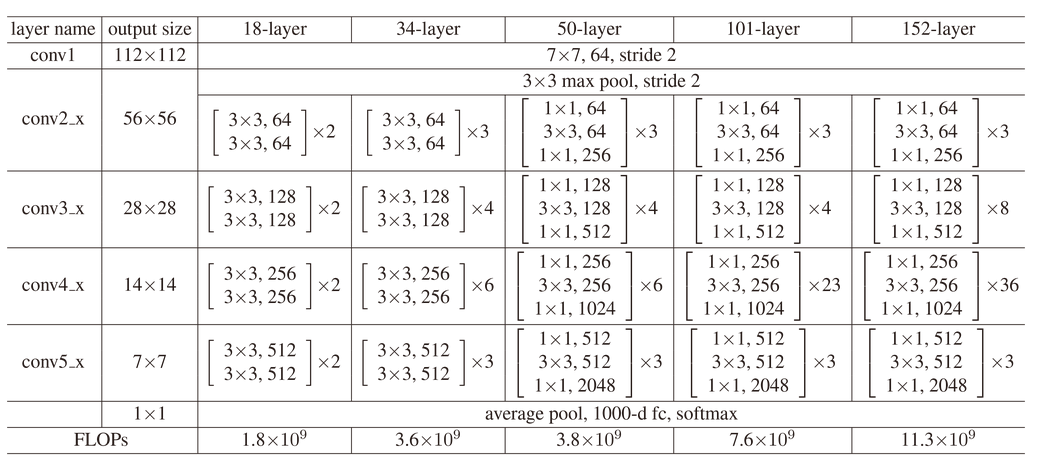
\includegraphics[width=5cm, height=4cm]{./pic/resnet_struct.png}
	\caption{resnet}
	\label{picresnet}
	\end{minipage}
	\begin{minipage}[t]{0.48\textwidth}
		\centering
		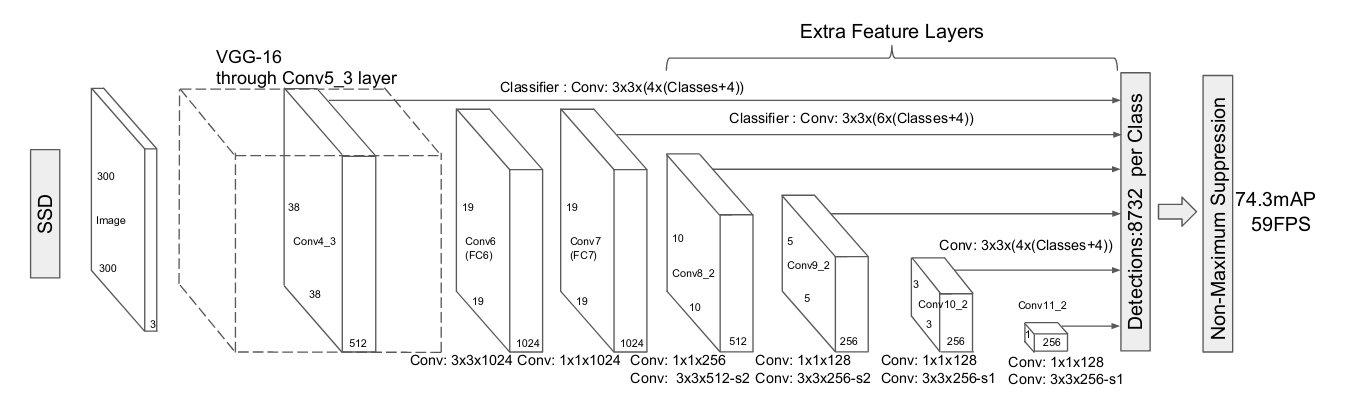
\includegraphics[width=5cm,height=4cm]{./pic/ssd.png}
		\caption{ssd}
		\label{picssd}
	\end{minipage}
\end{figure}

\begin{figure}[htbp]
	\centering
	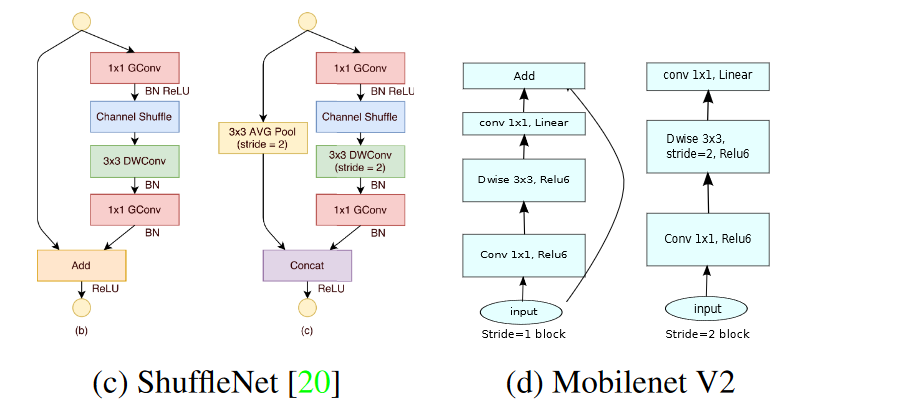
\includegraphics[width=8cm,height=6cm]{./pic/MobileNetV2.png}
	\caption{mobilenetv2}
	\label{picmobilenet}
\end{figure}


\subsubsection{backbone及改进}

Resnt的backbone由BasicBlock,Bottleneck, make\_res\_layer构成,前两个均是基本的残差结构,以卷积核大小分别为
1,3,1的顺序构件图,最后或接一下采样层,组成一个基础的残差block。
make\_res\_layer中重复构造残差模块,增加感受野和特征的复杂度。

backbone的改进主要有模型轻量和功能扩展。

这里主要说说resnet.py中引进的dcn,gcb和gen\_attention等功能模块。
从Bottleneck的\_inner\_forward可以看到,gen\_attention\_block加到kerner\_size=1,
kerner\_size=3组(组:卷积,归一化,激活)之后,
kerner\_size=1,planes扩展组之前。
gcb加到planes扩展组之后,然后才是下采样。因dcn是替换卷积算子,其参数和基本卷积相同,因此你可以任意替换conv2d,
只是试验表明,替换此处的kerner\_size=3组效果更好。

代码参数说明,主要和fpn对齐部分,在config中按照如下对齐方式更改即可。
\lstset{style=mystyle}
\begin{lstlisting}[language=Python]

@BACKBONES.register_module
class ResNet(nn.Module):
	arch_settings = {
		18: (BasicBlock, (2, 2, 2, 2)),    # (2, 2, 2, 2)各层残差块的重复数目
		34: (BasicBlock, (3, 4, 6, 3)),
		50: (Bottleneck, (3, 4, 6, 3)),
		101: (Bottleneck, (3, 4, 23, 3)),
		152: (Bottleneck, (3, 8, 36, 3))
	}
	def __init__(self,
					depth,
					in_channels=3,
					num_stages=4,
					strides=(1, 2, 2, 2),
					dilations=(1, 1, 1, 1),
					out_indices=(0, 1, 2, 3),
					style='pytorch',
					frozen_stages=-1,
					conv_cfg=None,
					norm_cfg=dict(type='BN', requires_grad=True),
					norm_eval=True,
					dcn=None,
					stage_with_dcn=(False, False, False, False),
					gcb=None,
					stage_with_gcb=(False, False, False, False),
					gen_attention=None,
					stage_with_gen_attention=((), (), (), ()),
					with_cp=False,
					zero_init_residual=True):
		super(ResNet, self).__init__()
	# num_stages:下采样特征层数目
	# strides:不同残差block的stride数
	# out_indices: 需要的特征层索引,对齐fpn
	# frozen_stages:冻结的残差层
	# stage_with_dcn,stage_with_gcb,stage_with_gen_attention均需要和fpn层对齐

	def forward(self, x):
		# 首先是两个下采样:kernel_size=7和maxpool,此时尺度为原始1/4
		x = self.conv1(x)
		x = self.norm1(x)
		x = self.relu(x)
		x = self.maxpool(x)
		# 然后是几个尺度减半的特征层 make_res_layer,对应fpn层
		outs = []
		for i, layer_name in enumerate(self.res_layers):
			res_layer = getattr(self, layer_name)
			x = res_layer(x)
			if i in self.out_indices:
				# out_indices 选取需要的层对应fpn层(通常index是连续的,除非数据特殊,刚好都只有一大一小物体)
				outs.append(x)
		return tuple(outs)
\end{lstlisting}



\subsection{Necks}
\begin{figure}[htbp]
	\centering
	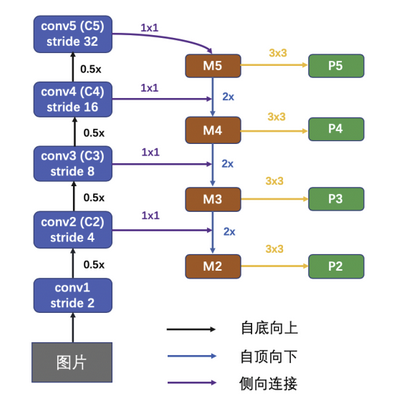
\includegraphics[width=5cm,height=4cm]{./pic/fpn.png}
	\caption{fpn}
	\label{picfpn}
\end{figure}

\begin{figure}[htbp]
	\centering
	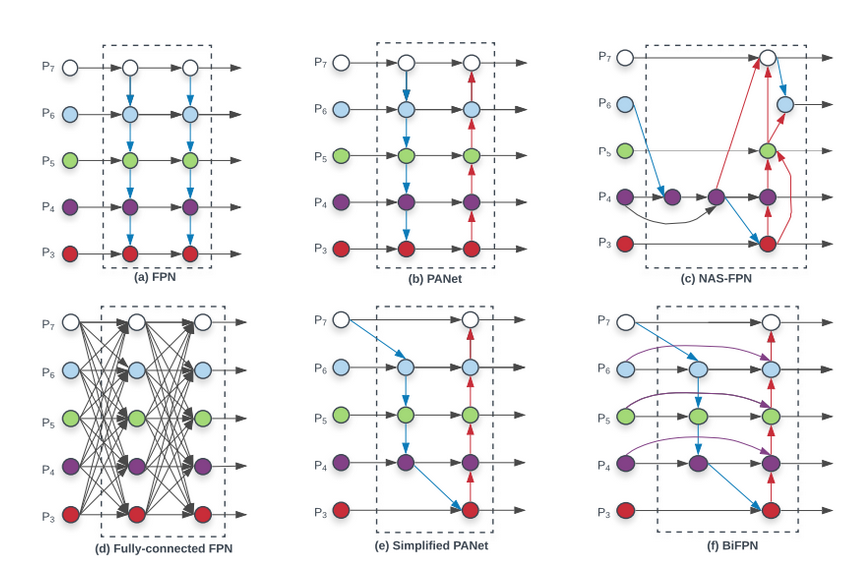
\includegraphics[width=7cm,height=4cm]{./pic/BiFPN.png}
	\caption{bifpn}
	\label{picbifpn}
\end{figure}


\subsubsection{多尺度结构}
FPN,BFPN BiFPN, HRFPN等。

\subsection{Heads}
Heads 主要包含了是三部分,anchor\_heads, bbox\_heads, mask\_heads,
anchor是two-stage的rpn部分或者one-stage的头部.最终的损失函数均在这里实现.

\subsubsection{AnchorHead}
\label{sub:anchorhead}
anchor head 主要包括AnchorGenerator, anchor\_target, 后者包含了assign,sample.因为不同尺度操作雷同,于是作者设计了一个公共函数multi
\_apply.这一小节主要说明以上函数,损失函数见\ref{sec:loss}.

AnchorGenerator类为不同特征层生成anchor,输入参数base\_size, scales, ratios分别表示:anchor在特征层上的基础大小(特征层相对于原图的stride),anchor在特征层上的尺度大小(可以多个,增加感受野),anchor在保持基础大小不变的情况下的长宽比.
len(scales)*len(ratios)即为一格的anchor个数.

比如输入图像大小(640*640), 选择(p2, p3)作为其特征层,则p2大小为(160*160),base\_ size=4,若设定ratios=[0.5,1.0,2.0], scales=[8, 16],则在p2上一格对应的base\_anchor的(w,h)为[(45.25,22.63),  (90.51, 45.25),
 (32.00, 32.00),  (64.00, 64.00), (22.63, 45.25),(45.25, 90.51)].其中$64=4*16*1,90.51=4*16*\sqrt{2}, 22.63=4*8/\sqrt{2}.$
 那么每一格所对应的6个base\_anchor相对于中心点的偏移量即为:
\lstset{style=mystyle}
\begin{lstlisting}[language=Python]
	
											[[-21.,  -9.,  24.,  12.],
											[-43., -21.,  46.,  24.],
											[-14., -14.,  17.,  17.],
											[-30., -30.,  33.,  33.],
											[ -9., -21.,  12.,  24.],
											[-21., -43.,  24.,  46.]]

\end{lstlisting}

因为这里都是相对于自身一格的偏移量,所有当要算在原图上的中心偏移量时,直接根据torch或者numpy的广播机制,
首先得到特征图在原图的网格坐标,然后和此相加,即得此特征层的所有all\_anchors.见grid\_anchors函数.
这里面涉及到一些操作技巧,比如:
\lstset{style=mystyle}
\begin{lstlisting}[language=Python]
ws = (w * w_ratios[:, None] * self.scales[None, :]).view(-1)
hs = (h * h_ratios[:, None] * self.scales[None, :]).view(-1)
\end{lstlisting}
包括nms,assign等部分都有很多细节操作,这些实现检测算法的基础函数,需要多加练,才能复现新的算法.可见\ref{sec:basefunc}.
如上不难看到,输入图像的所有anchor数量巨大.


模块anchor中还有一个anchor\_target文件,其主要是为了给设计的anchor标定label以及筛选anchor(便于优化等).

这里利用的anchor\_target\_single函数来解释multi\_apply函数:
\lstset{style=mystyle}
\begin{lstlisting}[language=Python]
from functools import partial
from six.moves import map, zip
def multi_apply(func, *args, **kwargs):
    pfunc = partial(func, **kwargs) if kwargs else func
    map_results = map(pfunc, *args)
	return tuple(map(list, zip(*map_results)))
\end{lstlisting}

partial 函数的功能就是:把一个函数的某些参数给固定住,返回一个新的函数(这里就是将**kwargs中的参数固定住).
当函数参数太多,需要固定某些参数时,可以使用 functools.partial 创建一个新的函数
map(function, sequence) ,对 sequence 中的 item 依次执行 function(item),并将结果组成一个 迭代器返回,
最后zip 并行循环.

在anchor\_target中
\lstset{style=mystyle}
\begin{lstlisting}[language=Python]
result = multi_apply(
         anchor_target_single,
         anchor_list,
         valid_flag_list,
         gt_bboxes_list,
         gt_bboxes_ignore_list,
         gt_labels_list,
         img_metas,
         target_means=target_means,
         target_stds=target_stds,
         cfg=cfg,
         label_channels=label_channels,
         sampling=sampling,
		 unmap_outputs=unmap_outputs)
\end{lstlisting}

是先将配置文件,采样与否的flag,anchor于gt\_box在映射空间(平移归一,放缩log)中各偏差量的
滑动平均处理(见core/bbox/transforms/bbox2delta函数最后一行)固定住.然后anchor\_target\_single
对*args参数:anchor\_list,gt\_bboxes\_list, img\_metas等并行处理.得到最终的label,bbox,正负样本index.这里 label\_weights用来记录筛选后的信息位置.

*args参数的说明:
\begin{itemize}
	\item anchor\_list:见anhor\_head中的get\_anchor函数,是一个list[list[Tensors]]结构,最外层是图片个数,再内一层是尺度个数,里面的Tensors的shape是[H*W*4, 4],其中H和W代表对应尺度特征图的高和宽.
	\item img\_metas有五个字段:ori/img/pad\_shape, scale\_factor, flip
	
\end{itemize}

在调用anchor\_target\_single函数之前:

\lstset{style=mystyle}
\begin{lstlisting}[language=Python]
num_imgs = len(img_metas)
assert len(anchor_list) == len(valid_flag_list) == num\_imgs
# anchor number of multi levels
# 选出第一张图的各个特征层的anchor数量,比如上面给的p2即为160*160*6,一格点对应的anhor shape为(6,4)
# 因为有多层,比如p2,p3,则[(160*160*4,4), (80*80*6,4)]
# 为images_to_levels函数,切片用:将所有以图片为第一维度的结果,转换成以特征图尺度个数为第一维度的结果(算loss)
num_level_anchors = [anchors.size(0) for anchors in anchor_list[0]]
# concat all level anchors and flags to a single tensor
#在调用multi\_apply之前需要将anchor\_list的不同层级的anchor cat在一起,最终变为list[Tensor]结构.
#最外层为图像个数.这样就能利用multi\_apply中的map在每张图上做做同样的操作了.
#将所有图的anchor合在一起
for i in range(num_imgs):
	assert len(anchor_list[i]) == len(valid_flag_list[i])
	anchor_list[i] = torch.cat(anchor_list[i])
	valid_flag_list[i] = torch.cat(valid_flag_list[i])
	# valid_flag_list结合meta信息,进一步筛选无效anhor(其实筛掉的很少)
\end{lstlisting}

anchor\_target\_single函数:主要涉及assign\_and\_sample,bbox2delta,
unmap四个函数.

assign\_and\_sample根据cfg从配置信息拿到对应的assign,sample类对象,
one-stage模型没有sample(不代表损失函数利用所有的anchor),sample主要为two-stage服务.

采样主要包含RandomSampler,OHEMSampler,InstanceBalancedPosSampler,IoUBalancedNegSampler,
均继承自BaseSampler为一抽象类,继承自它的的类必须完成
\_sample\_pos,\_sample\_neg两函数.按照python的语法,子类可以使用 raise NotImplementedError来避免不能实例化的问题.PseudoSampler即是如此,它重写了sample函数,该函数并没有做任何筛选.RandomSampler的意思自明,其他采样后补.
标定MaxIoUAssigner见\ref{sub:MaxIoUAssigner}.

bbox2delta 主要注意一点的是相对位置是相对于anchor的,所以除的是anchor的$w,h$
$$
d_x = (g_x - p_x) / p_w,
d_y = (g_y - p_y) / p_h,
d_w = \log(g_w / p_w),
d_h = \log(g_h / p_h).
$$
其中$x,y$是中心坐标.这里涉及到一些优化目标函数的变量的"变换"问题,比如这里若$g_w-p_w=1+\epsilon$,则$d_w=\epsilon$.如此似乎可以将其替换为$d_w=g_w/p_w-1$,实际上这样的效果可能还是不及$\log$,因为一开始它就将变化幅度压缩了.另外,相对位置的归一化差异是关键,比如人脸识别中,landmarks的优化,同常损失函数为欧氏距离,如何对变量进行处理?若是先预测bbox,再预测landmarks,可以相对于bbox的中心坐标做变换,若直接预测呢?

\subsubsection{SSDHead}
ssd结构的检测网络,目前已有ssd300,ssd512,结构细节参考\ref{backbone}. 从配置文件中可有看到,它没有neck,
因层级结构在backbone实现.

ssdhead继承自anchorhead,主要功能为处理多层级特征上的anchor构造和target标定与筛选,
基本的feauturemap上的acnhor生成由mmdet.core.
anchor中的AnchorGenerator完成,优化目标anchor由anhor\_target完成.
ssdhead中forward前向返回各层级对应的类别分数和坐标信息,loss函数则得到对应的损失函数,以字典的形式返回,最终求导时,汇总成一个值,同时也能计算各个部分损失函数的均值,方差,方便优化,debug.

此处的难点在于anchor的设定和target的标定,筛选.现就anchor这一块细说如下:

anchor基本介绍: anchor设计和caffe ssd anchor设计一致, 假设min\_size为$a$, max\_size为$b$, 则先生成ratio为1, 宽度和高度为$(a, a), (\sqrt{ab}$, 
$\sqrt{ab})$的两个anchor, ratio为$2, 1/2, 3, 1/3$则分别生成宽度和高度为$(a*\sqrt{ratio}, a/\sqrt{ratio})$的anchor, mmdetection中必须设定每一层的min\_size, max\_size, 因此ratios为$[2]$则对应4个anchor, ratios为$[2,3]$则对应6个anchor.

在init()函数中,先生成min\_size, max\_size, 注意它这里是必须要指定max\_size(和caffe SSD不同,无法生成奇数个anchor), 确保len(min\_size)=
len(max\_size), 调用AnchorGenerator()类生成了base\_anchors, 数量是6或者10,使用indices操作从6个anchor里选择$(0, 3, 1, 2)$或者从10个anchor里选择$(0, 5, 1, 2, 3, 4) $$\rightarrow$ 最终生成4个或者6个anchor.于在多个feature map上生成anchor,因此使用了一个for循环操作, 将anchor\_generator放入到anchor\_generatos[]中.


AnchorGenerator类, init()函数需要如下参数:

\begin{itemize}
	\item base\_size: 即设置的min\_size
	\item scales: 是$(1, \sqrt{max\_size / min\_size})$, 用来生成ratio为1的两个anchor
	\item ratios: 是$(1, 2, 1/2)$或者$(1, 2, 1/2, 3, 1/3)$
	\item ctr: ctr由stride生成, 是anchor的中心坐标, $(\frac{stride - 1}{2}, \frac{stride - 1}{2} ) $在gen\_base\_anchor()函数里, 使用上面的参数来计算base\_anchor, 计算流程如下:
	\begin{itemize}
		\item 根据ratios来计算h\_ratios和w\_ratios, 即上面所述的$(1 / \sqrt{ratios}$, $\sqrt{ratios}) $.
		\item 根据scales来计算base\_size, 一共有2个分别是$$(min\_size, \sqrt{min\_size * max\_size}) = min\_size * scales$$
		\item 计算anchors的宽度和高度, 只以宽度举例: $w = base\_size * w\_ratios$, 以ratios是$(1, 2, 1/2)$举例, base\_size shape为$(2, 1)$, w\_ratios shape为$(1, 3)$, 
		计算出的w是$(2, 3) $一共生成了6个anchor, 如果ratios是$(1, 2, 1/2, 3, 1/3)$, 则生成10个anchor (此处anchor数量和标准ssd anchor数量不一致 $\rightarrow$
		 再筛选(即ssd\_head.py中使用indices操作进行筛选))
	\end{itemize}
	
\end{itemize}


\subsubsection{RetinaHead}
后补。
\subsubsection{GuidedHead}
guided\_anchor\_head.py, ga\_retina\_head.py

\subsubsection{FCOSHead}
若其他人补。

\subsection{Losses}
\label{sec:loss}
\subsubsection{基本认识}

\href{https://arxiv.org/abs/1708.02002}{Fcoalloss}.
想像一下特征层上的锚框,远离gt的必然占绝大多数,围绕在gt周围的bbox有模棱两可的(正负),故有正负难易之分.FcoalLoss 是为解决难易样本的不平衡问题.公式如下:
\begin{equation}
	FL(p_t) = -\alpha_{t}(1-p_t)^{\gamma}log(p_t),\text{其中}
	p_t=\left\{
	\begin{aligned}
	&p & if y =1\\
	&1-p & else.
	\end{aligned}
	\right.
\end{equation}

$\alpha_t$缓解样本不平衡现象,$(1-p_t)^{\gamma}$为降低易分样本的损失值(考虑到易分样本比例高).
公式可以这样理解:对于正样本分对了,则$p_t->1$,$(1-p_t)^{\gamma}$有减缓效果,当分错了,即
$p_t << 0.5$,则$1-p_t >>0.5$,效果和CrossEntropy没差,对于负样本也是如此.因此起到压缩
图6中的左图右端,右图左端的效果.

\begin{figure}[htbp]
	\centering
	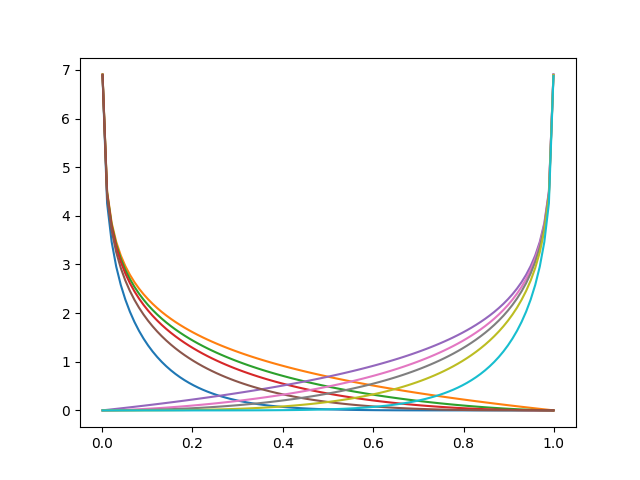
\includegraphics[width=5cm,height=3cm]{./pic/Focal_01.png}
	\caption{FcoalLoss}
\end{figure}

\href{https://arxiv.org/abs/1811.05181}{GHM}.
GHM算是对Fcoal改进,作者统计了样本的梯度信息,提出梯度均衡机制,让各种难度类型的样本有均衡的累计贡献.具体细节看论文即可.

\href{https://arxiv.org/abs/1908.03851}{IoULoss}.
\href{https://arxiv.org/abs/1711.00164}{BoundedIoULoss}.

\subsubsection{实现解析}
mmdet.models.losses里面实现了所有损失函数。

losses.utils有两个基本函数,weight\_reduce\_loss和weighted\_loss,前者将返回的损失向量点乘一权重向量,再分别求和或者算平均值。后者为一
装饰器,装饰你自己定义的损失函数,实现带权重效果。具体为先算自定义loss\_func,然后再weight\_reduce\_loss一下。其中weighted\_loss中的@functools.wraps
装饰的好处是返回的函数保持被装饰函数名字。接下来逐一说明各个损失函数。

CrossEntropyLoss,其理论来源有两点,信息论或极大似然估计,可参考花书。
pytorch官方文档给的公式,明显看出是极大似然的写法。注意实际运算是张(向)量的形式。
$\operatorname{loss}(x, \text { class })=-\log \left(\frac{\exp (x[\text { class }])}{\sum_{j} \exp (x[j])}\right)=
-x[\text { class }]+\log \left(\sum_{j} \exp (x[j])\right)$,增加权重因子为
$$\operatorname{loss}(x, \text { class })=
w e i g h t[\text { class }]
\left(-x[\text { class }]+\log \left(\sum_{j} \exp (x[j])\right)\right).$$
在cross\_entropy\_loss.py中实现了三种交叉熵损失函数,binary\_cross\_ent
ropy, mask\_cross\_entrop以及cross\_entropy,前两者相同点在于将标签扩展成one hot形式
然后调用F.binary\_cross\_entropy\_with\_logits函数,不同点为mask没有乘权重向量,cross\_entropy调用F.cross\_entropy,并被weight\_reduce\_loss了。
需要注意的点是,最终的CrossEntropyLoss中的loss\_weight参数是多任务中此Loss的权重。而weight\_reduce\_loss
中的weight是各类别的权重。可以说前者和样本平衡有关,后者和任务平衡有关。

SmoothL1Loss来源于FastRCNN,用于解决方框回归的不稳定问题(也许是优化速度),由L2,L1演变而来。
$$L_{1}=\begin{array}{l}
	0.5 x^{2}, \quad|x|<1 \\
	|x|-0.5, \quad x<-1 \text { or } x>1
	\end{array}$$
三者的关系,画个图其意自明:L2两边变化太快,对不好优化的anchor不友好(离群点),L1 0点不可导,Smooth两边较为平缓。
在smooth\_l1\_loss.py中,smooth\_l1\_loss被上述weighted\_loss装饰,
实现代码比较简单:
\lstset{style=mystyle}
\begin{lstlisting}[language=Python]
diff = torch.abs(pred - target)
loss = torch.where(diff < beta, 0.5 * diff * diff / beta,
				   diff - 0.5 * beta)
\end{lstlisting}
注意这里的where实现了分段函数,所以其含义自明。

BalancedL1Loss来自Libra R-CNN,为SmoothL1的改进。
改进函数为
$$
L_{b}(x)=\left\{\begin{array}{ll}
	\frac{\alpha}{b}(b|x|+1) \ln (b|x|+1)-\alpha|x| & \text { if }|x|<1 \\
	\gamma|x|+C & \text { otherwise }
	\end{array}\right.
$$
其梯度为:
$$
\frac{\partial L_{b}}{\partial x}=\left\{\begin{array}{ll}
	\alpha \ln (b|x|+1) & \text { if }|x|<1 \\
	\gamma & \text { otherwise }
	\end{array}\right.
$$
其中$b=e^{\frac{\gamma}{\alpha}}$,使得函数连续。容易得到在 $|x|<1$ 附近的梯度比SmoothL1要大。
具体分析可参考\href{https://zhuanlan.zhihu.com/p/64541760}{BalancedL1Loss},代码和SmoothL1一致,故析略。

Fcoalloss原理见上节,其扩展有\href{https://arxiv.org/pdf/1904.07850.pdf}{CenterNet},GHM系列。
因\_sigmoid\_focal\_loss由cpp,cu实现,故略(可看看debug版本)。 

GHMLoss有GHMC, GHMR,分别作用于分类,回归。原理查看论文或者参考\href{https://zhuanlan.zhihu.com/p/80594704}{GHM},
其主要思想是简单和特难的样本均进行抑制,也算是FocalLoss的改进,析码略。

剩下的IoULoss,BoundedIoULoss,GIoULoss等以iou的方式进行Box回归,含义自现。
三者的细致分析(各自优缺点及关系)看原始论文。代码上根据如下公式,即可容易写出。
Giou:
\begin{equation*}
\begin{array}{l}
	I o U=\frac{|A \cap B|}{|A \cup B|} \\
	G I o U=I o U-\frac{|C \backslash(A \cup B)|}{|C|}
	\end{array}
\end{equation*}其中$C$为$A, B$的闭包。
在iou\_loss.py中,最终的iou\_loss为$-log(ious)$, giou\_loss为$1-gious$
, boundedloss和SmoothL1Loss差不多,只是此时被求的变量$(dx,dy,dw,dh)$的编码方式变了。
具体关系如下:

论文中的分段函数为Huber loss
$
L_{\tau}(z)=\left\{\begin{array}{cc}
	\frac{1}{2} z^{2} & |z|<\tau \\
	\tau|z|-\frac{1}{2} \tau^{2} & \text { otherwise }
	\end{array}\right.
$
和SmoothL1类似,但代码用的是带了一个$\beta$因子的SmoothL1。

分量损失为
$
\text { cost }_{\mathrm{i}}=
2 L_{1}\left(1-\mathrm{I} \mathrm{o} \mathrm{U}_{\mathrm{B}}\left(i, b_{t}\right)\right)
, i \in \{x, y, w, h\}.$
原始的$L1$(见FasterRCNN)定义为
$$
\begin{aligned}
	&\operatorname{cost}_{x}=L_{1}\left(\frac{\Delta x}{w_{s}}\right)\\
	&\operatorname{cost}_{\mathrm{w}}=L_{1}\left(\ln \left(\frac{w}{w_{t}}\right)\right)
	\end{aligned}
$$
这里使用的
$\mathrm{IoU}_{\mathrm{B}}$定义为:
$$
\begin{array}{l}
	\operatorname{IoU}_{\mathrm{B}}\left(x, b_{t}\right)=\max \left(0, \frac{w_{t}-2|\Delta x|}{w_{t}+2|\Delta x|}\right) \\
	\operatorname{IoU}_{\mathrm{B}}\left(w, b_{t}\right)=\min \left(\frac{w}{w_{t}}, \frac{w_{t}}{w}\right)
	\end{array}.
$$
最终分别算出$x,y,w,h$的各自$IoU_B$"损失",作为最终损失的分量,带入SmoothL1分段函数中即可。


以上的代码中出现了new\_full,nonzero,numel,expand,where等常用函数。


\subsection{Detectors}
这节主要分析maskrcnn和reppoints,retinaFace三个算法.

\subsubsection{maskrcnn}
\label{maskrcnn}
以配置文件mask\_rcnn\_r50\_fpn\_1x.py为例说说twao\_stage的实现过程.
配合two\_stage的forward\_train()函数和配置文件,即可.

首先backbone为resnet50,(resnet系列结构参见\ref{picresnet}),
其以tuple形式返回4个stage的特征图,片段代码如下:
% \begin{figure}[htbp]
% 	\centering
% 	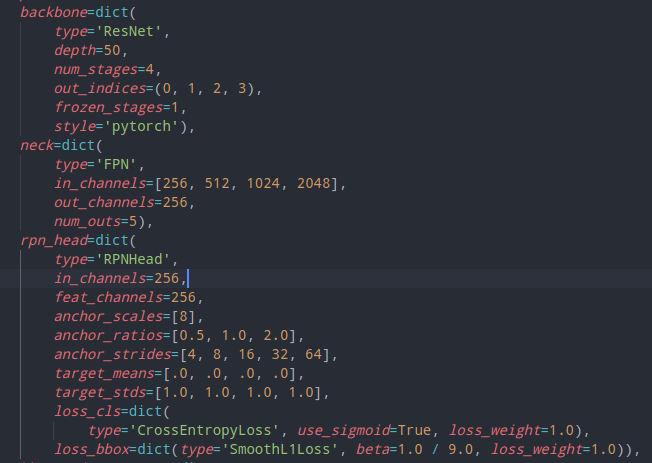
\includegraphics[width=5cm, height=4cm]{./pic/maskrcnn_50.png}
% 	\caption{config maskrcnn}
% \end{figure}
\lstset{style=mystyle}
\begin{lstlisting}[language=Python]

outs = []
for i, layer_name in enumerate(self.res_layers):
	res_layer = getattr(self, layer_name)
	x = res_layer(x)
	if i in self.out_indices:
		outs.append(x)

\end{lstlisting}

然后neck为fpn,结构参见\ref{picfpn},
fpn根据config中的out\_indices取出以resnet50输出的对应stage,分别构造输出channel维度统一的卷积算子,然后按照\ref{picfpn}所示融合方式进行不同尺度的特征融合,以元组形式输出结果.
在配置信息里有一条num\_outs=5,是为mask-rcnn在最顶层特征增加的最大池化特征输出.以上两块为提取特征,被extract\_feat整合在一块,

% \lstset{style=mystyle}
% \begin{lstlisting}[language=Python]
% 	for i in range(self.start_level, self.backbone_end_level):
% 		l_conv = ConvModule(
% 			in_channels[i],
% 			out_channels,
% 			1,
% 			conv_cfg=conv_cfg,
% 			norm_cfg=norm_cfg,
% 			activation=self.activation,
% 			inplace=False)
% 		fpn_conv = ConvModule(
% 			out_channels,
% 			out_channels,
% 			3,
% 			padding=1,
% 			conv_cfg=conv_cfg,
% 			norm_cfg=norm_cfg,
% 			activation=self.activation,
% 			inplace=False)

% 		self.lateral_convs.append(l_conv)
% 		self.fpn_convs.append(fpn_conv)

% \end{lstlisting}
紧接着forward\_train中包含了剩下的所有流程.
\begin{equation*}
	\begin{aligned}
		 rpn\_head \rightarrow rpn\_head.loss \rightarrow rpn\_head.get\_bboxes \rightarrow assign \rightarrow sample \\
		\rightarrow bbox\_roi\_extractor \rightarrow  bbox\_head \rightarrow bbox\_head.get\_target. \rightarrow bbox\_h\\
		ead.loss \rightarrow mask\_roi\_extractor \rightarrow mask\_head \rightarrow mask\_head.get\_target
	\end{aligned}
\end{equation*} 

这里梳理一下部分函数.

候选框层RPN,RPNHead继承AnchorHead, 它的几个核心操作都在anchor\_head.py中实现,主要包括get\_anchors, anchor\_target见\ref{sub:anchorhead},函数get\_bboxes结合配置参数从rpn前向得到的
2分类和位置预测结果中筛选出最终的proposals.

get\_bboxes中先通过self.anchor\_generators[i].grid\_anchors()这个函数取到所有的anchor\_boxs,再通过self.get\_bboxes\_single()根据rpn前向的结果选出候选框,
在self.get\_bboxes\_single()中,先在每个尺度上取2000(配置)个anchor出来,concat到一起作为该图像的anchor,对这些anchor boxs作nms(thr=0.7)就得到了所需的候选框.
需注意预测的bbox是对数化了的,在做iou计算之前需用delta2bbox()函数进行逆变换.bbox\_head中的bbox2roi类似.

得到的候选框最终由配置中train\_cfg的rcnn.assigner, rcnn.sampler进行标定和筛选,保持正负样本平衡和框的质量,方便优化.

MaxIoUAssigner:
\label{sub:MaxIoUAssigner}
\begin{adjustwidth}{1cm}{0cm}
\begin{itemize}
	\item[1.] 所有候选框置-1
	\item[2.] 将与所有gtbbox的iou小于neg\_iou\_thr置0
	\item[3.] iou大于pos\_iou\_thr的将其匹配
	\item[4.] 为了避免标定框无训练目标,将gtbbox匹配于与它iou最近的bbox(会导致部分正样本的匹配iou值很小).
\end{itemize}
\end{adjustwidth}


\lstset{style=mystyle}
\begin{lstlisting}[language=Python]
	# 交并比矩阵(n,m), gt=n, bboxes=m
	overlaps = bbox_overlaps(gt_bboxes, bboxes)
	# 每个bbox和所有gt的最大交并比,(m,)
	max_overlaps, argmax_overlaps = overlaps.max(dim=0)
	# 每个gt和所有bbox的最大交并比
	gt_max_overlaps, gt_argmax_overlaps = overlaps.max(dim=1)
	# 1将所有bbox赋值为-1,注意new_full操作
	assigned_gt_inds = overlaps.new_full(
			(num_bboxes, ), -1, dtype=torch.long)
	# 2交并比大于0同时小于负阈值的赋值为0
	assigned_gt_inds[(max_overlaps >= 0)
							 & (max_overlaps < self.neg_iou_thr)] = 0
	# 将与gt交并比大于正阈值的赋值为1(可能没有)
	pos_inds = max_overlaps >= self.pos_iou_thr
	assigned_gt_inds[pos_inds] = argmax_overlaps[pos_inds] + 1
	# 保证每个gt至少对应一个bbox
	# 遍历gt,将与gt最近(max(iou))的bbox,将gt的label赋值给此bbox

	for i in range(num_gts):
			if gt_max_overlaps[i] >= self.min_pos_iou:
				# 此判断较迷
				max_iou_inds = overlaps[i, :] == gt_max_overlaps[i]
				assigned_gt_inds[max_iou_inds] = i + 1 
				# 与gt最大iou的bbox 赋值为i+1

\end{lstlisting}

RandomSampler,保持设定的平衡比例,随机采样.

然后通过SingleRoIExtractor(roi\_extractors/single\_level.py)统一RoI
Align四个尺度且大小不同的的proposals,使其大小为7*7(bbox)或14*14
(mask).配置信息rpn\_head中的anchor\_strides为5个尺度,
包含了fpn额外加入的最大池化层,而bbox\_roi\_extractor的featmap\_strides却只包含四个尺度,表明只需对前四层进行align.
最终送入bbox head 和mask head做第二次优化(two stage).

RoIAlign在ops中,经cuda加速,详解待后.
其中roi\_extractors中的特征层级映射函数如下:
\lstset{style=mystyle}
\begin{lstlisting}[language=Python]
	def map_roi_levels(self, rois, num_levels):
	"""Map rois to corresponding feature levels by scales.
	 self.finest_scale = 56, 映射到0级的阈值
	$(0, 56, 56*2, 56*4, \infty) \rightarrow (0, 1, 2, 3)$
	bbox2roi变换后的rois

	Returns:
		Tensor: Level index (0-based) of each RoI, shape (k, )
		因不同层级对应不同的ROIAlign
	"""
	scale = torch.sqrt(
		(rois[:, 3] - rois[:, 1] + 1) * (rois[:, 4] - rois[:, 2] + 1))
	target_lvls = torch.floor(torch.log2(scale / self.finest_scale + 1e-6))
	target_lvls = target_lvls.clamp(min=0, max=num_levels - 1).long()
	# 这个变换在原始论文中有.
	return target_lvls
\end{lstlisting}

\subsubsection{RepPoints}
	利用DCN特性,实现了检测的结构点表示方式的优化.

\subsubsection{RetinaFace}
再说,和ssd重复较大。

\section{数据处理}
\label{sec:detail}
\subsection{检测分割数据}
看看配置文件,数据相关的有data dict,里面包含了train,val,test的路径信息,用于数据类初始化。
然后就是pipeline,将各个函数及对应参数以字典形式放到列表里面,是对pytorch原装的transforms+compose,
在检测,分割相关数据上的一次封装,使得形式更加统一。

从builder.py中build\_dataset函数能清晰的看到,构建数据有三种方式,ConcatDataset,RepeatDataset和从注册器中提取。

其中dataset\_wrappers.py中ConcatDataset和RepeatDataset意义自明。前者继承自pytorch原始的ConcatDataset,
将多个数据集整合到一起,将不同序列(可参考\href{https://docs.python.org/zh-cn/3/library/collections.abc.html}
{容器的抽象基类})的长度相加,\_\_getitem\_\_函数对应index替换一下。
后者就是单个数据类(序列)的多次重复。就功能来说,前者提高数据丰富度,后者可解决数据太少使得loading时间长的问题。
而与注册相关的,被注册的数据类在datasets下大家熟知的数据类型的py文件中。基类为custom.py中的CustomDataset,coco继承自它,
cityscapes继承自coco,xml\_style的XMLDataset继承CustomDataset,然后wider\_face,voc均继承自XMLDataset。因此这里先分析一下CustomDataset。


CustomDataset 记录数据路径等信息,解析标注文件,将每一张图的所有信息以字典作为数据结构存在results中。然后进入pipeline,也即数据增强相关操作。
从下面代码可以清晰的看到。这里数据结构的选取需要注意一下,字典结构,在数据增强库albu中也是如此处理,因此可以快速替换albu中的算法。
另外每个数据类增加了各自的evaluate函数。evaluate基础函数在mmdet.core.evaluation中,后做补充。

\lstset{style=mystyle}
\begin{lstlisting}[language=Python]
	self.pipeline = Compose(pipeline)   
	# Compose是实现了__call__方法的类,其作用是使实例能够像函数一样被调用,同时不影响实例本身的生命周期
def pre_pipeline(self, results):
	# 扩展字典信息
	results['img_prefix'] = self.img_prefix
	results['seg_prefix'] = self.seg_prefix
	results['proposal_file'] = self.proposal_file
	results['bbox_fields'] = []
	results['mask_fields'] = []
	results['seg_fields'] = []

def prepare_train_img(self, idx):
	img_info = self.img_infos[idx]
	ann_info = self.get_ann_info(idx)
	# 基本信息,初始化字典
	results = dict(img_info=img_info, ann_info=ann_info)
	if self.proposals is not None:
		results['proposals'] = self.proposals[idx]
	self.pre_pipeline(results)
	return self.pipeline(results)    # 数据增强

def __getitem__(self, idx):
	if self.test_mode:
		return self.prepare_test_img(idx)
	while True:
		data = self.prepare_train_img(idx)
		if data is None:
			idx = self._rand_another(idx)
			continue
		return data
\end{lstlisting}

mmdet的数据处理,字典结构,pipeline,evaluate是三个关键部分。其他所有类的文件解析部分,数据筛选等,看看即可。
因为我们知道,pytorch读取数据,是将序列转化为迭代器后进行io操作的。所以在dataset下除了pipelines外还有loader
文件夹,里面实现了分组,分布式分组采样方法,以及调用了mmcv中的collate函数,且build\_dataloader封装的DataLoader最后在
train\_detector中被调用,这部分将在后面补充,这里说说pipelines。所有pipelines的注册函数在\_\_init\_\_.py中可见。

返回maskrcnn的配置文件,可以看到,训练和测试的不同,LoadAnnotations,MultiScaleFlipAug,DefaultFormatBundle和Collect。
虽然测试没有LoadAnnotations,实际上根据前面的CustomDataset可知道,它仍然需要标注文件。这和inference的pipeline是不同的。

\lstset{style=mystyle}
\begin{lstlisting}[language=Python]
# 序列中的dict可以随意删减,增加,所谓数据增强调参
train_pipeline = [
    dict(type='LoadImageFromFile'),
    dict(type='LoadAnnotations', with_bbox=True, with_mask=True),
    dict(type='Resize', img_scale=(1333, 800), keep_ratio=True),
    dict(type='RandomFlip', flip_ratio=0.5),
    dict(type='Normalize', **img_norm_cfg),
    dict(type='Pad', size_divisor=32),
    dict(type='DefaultFormatBundle'),
    dict(type='Collect', keys=['img', 'gt_bboxes', 'gt_labels', 'gt_masks']),
]

test_pipeline = [
    dict(type='LoadImageFromFile'),
    dict(
        type='MultiScaleFlipAug',
        img_scale=(1333, 800),
        flip=False,
        transforms=[
            dict(type='Resize', keep_ratio=True),
            dict(type='RandomFlip'),
            dict(type='Normalize', **img_norm_cfg),
            dict(type='Pad', size_divisor=32),
            dict(type='ImageToTensor', keys=['img']),
            dict(type='Collect', keys=['img']),
        ])
]
\end{lstlisting}
这些所有操作被Compose串联起来(列表是序列结构)。

\lstset{style=mystyle}
\begin{lstlisting}[language=Python]
@PIPELINES.register_module
class Compose(object):

	def __init__(self, transforms):
		assert isinstance(transforms, collections.abc.Sequence)
		self.transforms = []
		for transform in transforms:
			if isinstance(transform, dict):
				transform = build_from_cfg(transform, PIPELINES)
				self.transforms.append(transform)
			elif callable(transform):
				self.transforms.append(transform)
			else:
				raise TypeError('transform must be callable or a dict')

	def __call__(self, data):
		for t in self.transforms:
			data = t(data)
			if data is None:
				return None
		return data
\end{lstlisting}
上面代码能清晰的看到,配置文件中pipeline中的字典传入build\_from\_cfg函数,逐一实现了各个增强类。
扩展的增强类均需实现\_\_call\_\_方法,这和pytorch原始方法是一致的。

\lstset{style=mystyle}
\begin{lstlisting}[language=Python]
def build_from_cfg(cfg, registry, default_args=None):
	assert isinstance(cfg, dict) and 'type' in cfg
	assert isinstance(default_args, dict) or default_args is None
	args = cfg.copy()
	obj_type = args.pop('type')
	if mmcv.is_str(obj_type):
		# 从注册类中拿出obj_type类
		obj_cls = registry.get(obj_type)
		if obj_cls is None:
			raise KeyError('{} is not in the {} registry'.format(
				obj_type, registry.name))
	elif inspect.isclass(obj_type):
		obj_cls = obj_type
	else:
		raise TypeError('type must be a str or valid type, but got {}'.format(
			type(obj_type)))
	if default_args is not None:
		# 增加一些新的参数
		for name, value in default_args.items():
			args.setdefault(name, value)
	return obj_cls(**args)    # **args是将字典解析成位置参数(k=v)。
\end{lstlisting}

有了以上认识,重新梳理一下pipelines的逻辑,由三部分组成,load,transforms,和format。
load相关的LoadImageFromFile,LoadAnnotations都是字典results进去,字典results出来。具体代码看下便知,
LoadImageFromFile增加了'filename','img','img\_shape','ori\_shape','pad\_shape',
'scale\_factor','img\_norm\_cfg'字段。其中img是numpy格式。LoadAnnotations从results['ann\_info']中解析出bboxs,masks,labels等信
息。注意coco格式的原始解析来自pycocotools,包括其评估方法,这里关键是字典结构。
transforms中的类作用于字典的values,也即数据增强。format中的DefaultFormatBundle是将数据转成mmcv扩展的容器类格式DataContainer。
另外Collect会根据不同任务的不同配置,从results中选取只含keys的信息生成新的字典,具体看下该类帮助文档。
这里看一下从numpy转成tensor的代码:

\lstset{style=mystyle}
\begin{lstlisting}[language=Python]
def to_tensor(data):
    """Convert objects of various python types to :obj:`torch.Tensor`.

    Supported types are: :class:`numpy.ndarray`, :class:`torch.Tensor`,
    :class:`Sequence`, :class:`int` and :class:`float`.
    """
    if isinstance(data, torch.Tensor):
        return data
    elif isinstance(data, np.ndarray):
        return torch.from_numpy(data)
    elif isinstance(data, Sequence) and not mmcv.is_str(data):
        return torch.tensor(data)
    elif isinstance(data, int):
        return torch.LongTensor([data])
    elif isinstance(data, float):
        return torch.FloatTensor([data])
    else:
        raise TypeError('type {} cannot be converted to tensor.'.format(
			type(data)))
	以上代码告诉我们,基本数据类型,需掌握。
\end{lstlisting}

那么DataContainer是什么呢?它是对tensor的封装,将results中的tensor转成DataContainer格式,实际上只是增加了几个property函数,
cpu\_only,stack,padding\_value,pad\_dims,其含义自明,以及size,dim用来获取数据的维度,形状信息。
考虑到序列数据在进入DataLoader时,需要以batch方式进入模型,那么通常的collate\_fn会要求tensor数据的形状一致。但是这样不是很方便,
于是有了DataContainer。它可以做到载入GPU的数据可以保持统一shape,并被stack,也可以不stack,也可以保持原样,或者在非batch维度上做pad。
当然这个也要对default\_collate进行改造,mmcv在parallel.collate中实现了这个。

也许可以看看通常的collate\_fn,它是DataLoader中将序列dataset组织成batch大小的函数。

\lstset{style=mystyle}
\begin{lstlisting}[language=Python]
def collate_fn_1(batch):
	# 这是默认的,明显batch中包含相同形状的img\_tensor和label
	return tuple(zip(*batch))
	
def coco_collate_2(batch):
	# 传入的batch数据是被albu增强后的(字典结构)
    imgs = [s['image'] for s in batch]    # tensor, h, w, c->c, h, w , handle at transform in __getitem__
    annots = [s['bboxes'] for s in batch]
    labels = [s['category_id'] for s in batch]

	# 以当前batch中图片annot数量的最大值作为标记数据的第二维度值,空出的就补-1。
    max_num_annots = max(len(annot) for annot in annots)
    annot_padded = np.ones((len(annots), max_num_annots, 5))*-1

    if max_num_annots > 0:
        for idx, (annot, lab) in enumerate(zip(annots, labels)):
            if len(annot) > 0:
                annot_padded[idx, :len(annot), :4] = annot
				# 不同模型,损失值计算可能不同,这里ssd结构需要改为xyxy格式并且要做尺度归一化
				# 这一步完全可以放到\_\_getitem\_\_中去,只是albu的格式需求问题。
                annot_padded[idx, :len(annot), 2] += annot_padded[idx, :len(annot), 0]    #  xywh-->x1,y1,x2,y2 for general box,ssd target assigner
                annot_padded[idx, :len(annot), 3] += annot_padded[idx, :len(annot), 1]    # contains padded -1 label
                annot_padded[idx, :len(annot), :] /=  640    # priorbox for ssd primary target assinger
                annot_padded[idx, :len(annot), 4] = lab
	return torch.stack(imgs, 0), torch.FloatTensor(annot_padded)
	
def detection_collate_3(batch):
    targets = []
    imgs = []
    for _, sample in enumerate(batch):
        for _, img_anno in enumerate(sample):
            if torch.is_tensor(img_anno):
                imgs.append(img_anno)
            elif isinstance(img_anno, np.ndarray):
                annos = torch.from_numpy(img_anno).float()
                targets.append(annos)
    return torch.stack(imgs, 0), targets    # 做了stack, DataContainer可以不做stack
\end{lstlisting}

以上就是数据处理的相关内容。
最后再用DataLoader封装拆成迭代器,其相关细节,sampler等就略去了。
\lstset{style=mystyle}
\begin{lstlisting}[language=Python]
data_loader = DataLoader(
	dataset,
	batch_size=batch_size,
	sampler=sampler,
	num_workers=num_workers,
	collate_fn=partial(collate, samples_per_gpu=imgs_per_gpu),
	pin_memory=False,
	worker_init_fn=init_fn,
	**kwargs)
\end{lstlisting}


\section{FP16}
模型预测加速等.


\section{训练pipeline}
\label{trainpipeline}
\subsection{训练逻辑}
图见\ref{trainpipe_pic}注意它的四个层级.主要查看api/train.py, mmcv中的runner相关文件.
% 这里说说非分布训练模式\_non\_dist\_train.
主要两个类:Runner和Hook
Runner将模型,批处理函数batch\_pro
cessor,优化器作为基本属性,是为训练过程中记录相关节点信息,
这些信息均被记录在mode,\_hooks,\_epoch,\_iter,\_inner\_iter,\_max\_epochs,\_max\_
iters中.从而实现训练过程中插入不同的操作,也即各种hook.
理清训练流程只需看Runner的成员函数run.在run里会根据mode按配置(workflow)epoch循环调用train和val函数,
跑完所有的epoch.其中train代码如下:
\lstset{style=mystyle}
\begin{lstlisting}[language=Python]
 def train(self, data_loader, **kwargs):
	self.model.train()
	self.mode = 'train'    # 改变模式
	self.data_loader = data_loader
	self._max_iters = self._max_epochs * len(data_loader)    # 最大batch循环次数
	self.call_hook('before_train_epoch')    # 根据名字获取hook对象函数
	for i, data_batch in enumerate(data_loader):
		self._inner_iter = i    # 记录训练迭代轮数
		self.call_hook('before_train_iter')    # 一个batch前向开始
		outputs = self.batch_processor(
			self.model, data_batch, train_mode=True, **kwargs)
		self.outputs = outputs
		self.call_hook('after_train_iter')    # 一个batch前向结束
		self._iter += 1    # 方便resume时,知道从哪一轮开始优化

	self.call_hook('after_train_epoch')    # 一个epoch结束
	self._epoch += 1    # 记录训练epoch状态,方便resume

\end{lstlisting}

上面让人困惑的是hook函数,
hook函数继承自mmcv的Hook类,其默认了6+8+4个函数,也即\ref{trainpipe_pic}所示的6个层级节点,
外加2*4个区分train和val的节点记录函数,以及4个边界检查函数.
从train.py中容易看出,在训练之前,已经将需要的hook函数注册到Runner的self.\_hook中了,包括从配置文件解析的优化器,学习率调整函数,模型保存,
一个batch的时间记录等(注册hook算子在self.\_hook中按优先级升序排列).
于是只需理解call\_hook函数即可.
\lstset{style=mystyle}
\begin{lstlisting}[language=Python]
def call_hook(self, fn_name):
	for hook in self._hooks:
		getattr(hook, fn_name)(self)
\end{lstlisting}

如上看出,在训练的不同节点,将从注册列表中调用实现了该节点函数的类成员函数.比如
\lstset{style=mystyle}
\begin{lstlisting}[language=Python]
class OptimizerHook(Hook):

    def __init__(self, grad_clip=None):
        self.grad_clip = grad_clip

    def clip_grads(self, params):
        clip_grad.clip_grad_norm_(
            filter(lambda p: p.requires_grad, params), **self.grad_clip)

    def after_train_iter(self, runner):
        runner.optimizer.zero_grad()
        runner.outputs['loss'].backward()
        if self.grad_clip is not None:
            self.clip_grads(runner.model.parameters())
        runner.optimizer.step()
\end{lstlisting}
将在每个train\_iter后实现反向传播和参数更新.

学习率优化相对复杂一点,其基类LrUpdaterHook,实现了before\_run, before\_train\_epoch, before\_train\_iter三个hook函数,意义自明.
这里选一个余弦式变化,稍作说明:

\lstset{style=mystyle}
\begin{lstlisting}[language=Python]
class CosineLrUpdaterHook(LrUpdaterHook):

    def __init__(self, target_lr=0, **kwargs):
        self.target_lr = target_lr
        super(CosineLrUpdaterHook, self).__init__(**kwargs)

    def get_lr(self, runner, base_lr):
        if self.by_epoch:
            progress = runner.epoch
            max_progress = runner.max_epochs
        else:
            progress = runner.iter
            max_progress = runner.max_iters
        return self.target_lr + 0.5 * (base_lr - self.target_lr) * \
			(1 + cos(pi * (progress / max_progress)))
\end{lstlisting}
从get\_lr可以看到,学习率变换周期有两种,epoch->max\_epoch,或者更大的iter->max\_iter,后者表明一个epoch内不同batch的学习率可以不同,因为没有什么理论,所有这两种方式都行.
其中base\_lr为初始学习率,target\_lr为学习率衰减的上界,而当前学习率正如函数的返回表达式.

\section{更改模型}
\subsection{增加模块}
本身就包含了很多更改配置文件。
\subsection{模型瘦身}
替换backbone。

\section{抽离模型}
\subsection{retinanet\_resnet18}
主要注意点。

\section{新增模型}
\subsection{centernet}
直接抽离一个就行了。

\section{numpy,torch某些基础函数}
\label{sec:basefunc}
\subsection{损失函数部分}
torch相关:new\_full,nonzero,numel,expand,where见损失函数一节。
\subsection{模型实现部分}
待补。
\subsection{数据类部分}
待补。

\section{计划}
\begin{itemize}
	\item [0.] datasets
	\item [1.] 更改模型
	\item [2.] 抽离模型
	\item [3.] 新增模型centernet 
	\item [6.] ops中的ROIAlign,DCN
	\item [7.] 检测模型的简略综述
\end{itemize}

\section{检测模型的简略综述}
检测算法是由一些基本的组件组合而成.这也是mmdection出现的原因.这章节会在不同算法系列中总结一些基础组件,最后再做个提取.
\subsection{通用物体检测}
按照物体编码方式可分为三类.矩形编码(anchor机制),结构点编码(RepPoints)和所有点编码(mask).
\subsubsection{Yolo系列}
yolo相对孤立,v1就不说了,v2,v3基本思想还是来源于resnet,fpn,ssd等.
代码可参考 \href{https://github.com/ultralytics/yolov3}{yolov3}.

与SSD的不同之处:
\begin{itemize}
	\item 根据数据聚类9个先验框,分成3个尺度,分别作为三个检测层的 base anchor.
	\item 因为网络结构只有卷积和池化,所以可以做多尺度输入320-608,steps=32.
	\item 基础网络DarkNet19,53较resnet更为轻量,主要是$1*1$卷积的大量使用.
	\item 多尺度的处理方式是在每个尺度上均计算一次检测(yolo layer),这和ssd合并起来做统一处理不同.
	\item 框回归编码不同(相对于网格中心的偏移量,物体由一个中心网格预测,当物体重合度高时,此假设不成立).
	\item 网络结构实现方式大多采用配置文件解析(DarkNet).
\end{itemize}

\subsubsection{SSD系列}
ssd是第一个包含了几乎所有的检测组件的算法(各种检测算法的所有组件集),故能在后续的发展中多次被更改,
用于其他任务中,比如ctpn,textb
oxes++,faceboxes等.代码可参考:\href{https://github.com/sgrvinod/a-PyTorch-Tutorial-to-Object-Detection}{SSD-Tutorial}手把手教你实现ssd,
以及相关原理讲解. \href{https://github.com/amdegroot/ssd.pytorch}{ssd.pytorch} 
最先看的ssd源码,简洁完完整.
\href{https://github.com/lufficc/SSD}{maskrcnn-benchmark风格版ssd}.

原始SSD:

\begin{itemize}
	\item 多尺度
	\begin{itemize}
		\item 不同尺度的feature map上生成anchor(比如:$300**2-> 38**2*4+19**2*6+10**2*6+5**2*6+3**2*4+1**2*4$),进行位置回归和类别判断.
		\item 一个$m*n$大小的feature map,若每个cell(可以理解成物体的离散表示点)分配$k$个anchor,则每个cell输出$(c+4)*k*m*n$个预测值(class, box relative offset).
		\item 注意每个cell其实是一个向量,长度为 channel of feature map,可以理解成一个物体的某一部分(或全部)的向量表示或者整体表示的一部分.
		\item 事实上这里完成了两个任务,分类和位置回归,所以cell向量可能具有分段表示功效(这和权重共享是不矛盾的,共享的权重可能就具有可分离性). 
		\item anchor计算损失函数前的有效编码:首先中心坐标在特征层上归一化(等同于相对于原图的归一化),尺度根据原图尺寸以及当前特征图相对原图的尺寸进行设计,比如第一特征层相对于原图的0.1,然后计算相对偏移量以及坐标和尺度的"等效"处理,尺度求对数.
	\end{itemize}

	\item 数据增强
	\begin{itemize}
		\item DistortImage: 修改图像本身的brightness, contrast, saturation, hue, reordering channels.
		\item ExpandImage: 将DistortImage的图片用像素0进行扩展,同时以黑边的左上角为原点计算$[0,1]$的bbox的左上角和右下角两个点坐标.
		\item BatchSampler: sampled\_bboxes的值是随机在$[0,1]$上生成的bbox,并且和某个gt\_bboxes的IOU在$[min, max]$之间
		\item resize 到固定大小$300*300$,label也同时线性缩放.
		\item 以0.5概率随机水平翻转, 或者crop等
	\end{itemize}

	\item 样本平衡
	\begin{itemize}
		\item 难例挖掘,正负样本1:3等.我的理解是制造更有效的优化空间(anchor是让优化空间变得合理).
	\end{itemize}
	
	\item 损失函数 
	\begin{itemize}
		\item 利用GT box 给个生成的8732(可变)anchor打标签,筛选出有效优化对象,计算分类和回归值.
	\end{itemize}

	\item 后处理
	\begin{itemize}
		\item NMS, Soft-NMS, OHEM
	\end{itemize}

\end{itemize}

以上五部分均是以后论文的改进点.比如特征提取基础结构,采用其他有效的分类模型resnet,或者轻量级的mobilenet等,或者替换在新的结构上替换一些结构组成算子,卷积,激活,BN等操作. 比如多尺度的FPN类似思想,融合不同特征层,这在一定程度上解决了重复框,小物体问题(将同一物体的不同尺度表达进行融合,当然能减缓底层表达能力不足的现象).这些有FSSD,RSSD(没有必要都要去看,检测类的文章,理清基本组件,花时间分析组件功能,做实验验证想法,就ok了)等.数据增强的方式各不相同,主要是提高数据的丰富性,增加模型的泛化能力,这个属于工程问题,基本方法都来源于传统的图像处理.样本平衡的扩展可参考mmdetection,用制造更有效的优化空间来理解,就可以随意发挥了.

具体案例:

FaceBoxes:

textboxes++:


\subsubsection{Fast RCNN系列}
Mask R-CNN:

\href{https://github.com/facebookresearch/maskrcnn-benchmark}{maskrcnn-benchmark}能学习的东西都在这里面了(仔细研读3遍). 
Mask R-CNN = Faster R-CNN  with FCN on ROIs.其主要流程参见\ref{maskrcnn}.ROI Align原理:
去掉了图像下采样到特征图的坐标量化,保持分数坐标,同时ROI分格池化时,对格子的坐标也取消量化,从而减少了坐标的二度漂移.若两次量化,最坏的情况,下采样5次,会有近64的位置偏移,这样会漏掉小目标.最后的池化采用双线性插值,原理就是每个点的像素值是其临近4个像素点的距离权重平均.

Cascade RCNN发现只有proposal自身的阈值和训练器的训练阈值较为接近时,训练器的性能才最好.
\subsubsection{Anchor Free 系列}
FCOS

\subsection{总结}


\end{document}